\whiteBGstarBegin
\setcounter{section}{0}
\section{Lăng kính}
\begin{enumerate}[label=\bfseries Câu \arabic*:]
	
		\item \mkstar{1} 
		
		\cauhoi{
			
			Lăng kính được cấu tạo bằng khối chất trong suốt, đồng chất, thường có dạng hình lăng trụ. Tiết diện thẳng của lăng kính hình
			\begin{mcq}(4)
				\item tròn.
				\item elip.
				\item tam giác.
				\item chữ nhật.
			\end{mcq}
		}
		
		\loigiai{
			
			\textbf{Đáp án: C.}
			
			Vì lăng kính thường có dạng hình lăng trụ nên tiết diện thẳng của lăng kính là hình tam giác.
		}
		\item \mkstar{1} 
	
	\cauhoi{
		
		Điều nào sau đây là đúng khi nói về lăng kính?
		\begin{mcq}
			\item Lăng kính là một khối chất trong suốt hình lăng trụ đứng, có tiết diện thẳng là một hình tam giác
			\item Góc chiết quang của lăng kính luôn nhỏ hơn $90^\circ$.
			\item Hai mặt bên của lăng kính luôn đối xứng nhau qua mặt phẳng phân giác của góc chiết quang.
			\item Tất cả các lăng kính chỉ sử dụng hai mặt bên cho ánh sáng truyền qua.
		\end{mcq}
	}
	
	\loigiai{
		
		\textbf{Đáp án: A.}
		
		A - đúng
		
		B - sai vì: góc chiết quang A có thể lớn hơn 
		$90^\circ.$
		
		C - sai vì: chỉ có lăng kính tam giác cân hoặc tam giác đều thì hai mặt bên của lăng kính mới đối xứng nhau qua mặt phân giác cảu góc chiết quang
		
		D - sai
	}
	\item \mkstar{1} 
	
	\cauhoi{
		
		Lăng kính phản xạ toàn phần là một khối lăng trụ thủy tinh có tiết diện thẳng là
		\begin{mcq} (2)
			\item một tam giác vuông cân.
			\item một hình vuông.
			\item một tam giác đều.
			\item một tam giác bất kì.
		\end{mcq}
	}
	
	\loigiai{
		
		\textbf{Đáp án: A}
		
		Lăng kính phản xạ toàn phần là một khối lăng trụ thủy tinh có tiết diện thẳng là một tam giác vuông cân.
	}
	
	\item \mkstar{1} 
	
		\cauhoi {Chọn câu trả lời \textbf{sai}?
	\begin{mcq}
		\item Lăng kính là môi trường trong suốt đồng tính và đẳng hướng được giới hạn bởi hai mặt phẳng không song song.
		\item Tia sáng đơn sắc qua lăng kính sẽ luôn luôn bị lệch về phía đáy.
		\item Tia sáng không đơn sắc qua lăng kính thì chùm tia ló sẽ bị tán sắc.
		\item Góc lệch của tia đơn sắc qua lăng kính là $D=i+i'-A$.
	\end{mcq}
	}
	
	\loigiai{
		\textbf{Đáp án: B.}
		
		A, C, D - đúng
		
		B- sai vì: Khi ánh sáng truyền từ môi trường có chiết suất lớn hơn chiết suất của lăng kính thì tia ló sẽ lệch về phía đỉnh
	}

		\item \mkstar{1} 
	
	\cauhoi{
		
		Điều nào sau đây là đúng khi nói về lăng kính và đường đi của một tia sáng qua lăng kính?
		\begin{mcq}
			\item Tiết diện thẳng của lăng kính là một tam giác cân.
			\item Lăng kính là một khối chất trong suốt hình lăng trụ đứng, có tiết diện thẳng là một hình tam giác.
			\item Mọi tia sáng khi quang lăng kính đều khúc xạ và cho tia ló ra khỏi lăng kính.	
			\item Cả  A và C đều đúng.
		\end{mcq}
		
	}
	
	\loigiai{
		
		\textbf{Đáp án: B.}
		
		A- sai vì tiết diện thẳng của lăng kính có thể là tam giác cân có thể làm tam giác thường, có thể là  tam giác vuông , ...
		
		B- đúng
		
		C- sai vì không phải mọi tia sáng qua lăng kính đều cho tia ló ra khỏi lăng kính.
	}
	
	\item \mkstar{2} 
	
	\cauhoi{
		
		Chiếu một chùm tia sáng đỏ hẹp coi như một tia sáng vào mặt bên của một lăng kính có tiết diện thẳng là tam giác cân ABC có góc chiết quang $A = 8^\circ$ theo phương vuông góc với mặt phẳng phân giác của góc chiết quang tại một điểm tới rất gần A. Biết chiết suất của lăng kính đối với tia đỏ là $n_\text{đ}=\text{1,5}$. Góc lệch của tia ló so với tia tới là
		
		\begin{mcq}(4)
			\item $2^\circ$.
			\item $8^\circ$.
			\item $4^\circ$.
			\item $12^\circ$.
		\end{mcq}
		
	}
	
	\loigiai{
		\textbf{Đáp án: C.}
		
		Góc lệch của tia tới so với tia ló
		
		$$D = A(n-1) = 4^\circ.$$
	}
	

	\item \mkstar{2}
	
	\cauhoi{
		
		Cho một chùm tia sáng chiếu vuông góc đến mặt AB của một lăng kính ABC vuông góc tại A và góc ABC bằng $30^\circ$, làm bằng thủy tinh chiết suất $n = \text{1,3}$. Tính góc lệch của tia ló so với tia tới.  
		
		\begin{mcq}(4)
			\item $\text{40,5}^\circ$.
			\item $\text{20,2}^\circ$.
			\item $\text{19,5}^\circ$.  	
			\item $\text{10,5}^\circ$. 
		\end{mcq}
	}
	
	\loigiai{
		\textbf{Đáp án: D.}
		
		Ta có góc $i_1 =0^\circ \Rightarrow r_1 = 0^\circ.$
		
		Góc chiết quang B
		
		$$B  = r_1 + r_2 \Rightarrow r_2 = 30^\circ.$$
		
		Áp dụng định luật khúc xạ ánh sáng
		
		$$\sin i_2 = n \sin r_2 \Rightarrow r_2 = \text{40,5}^\circ.$$
		
		Góc lệch giữa tia ló và tia tới
		
		$$D = i_2 -r_2 = \text{10,5}^\circ.$$
		
		
	}
	
	\item \mkstar{2}
	
	\cauhoi{
		
		Sử dụng hình vẽ về đường đi của tia sáng qua lăng kính có góc chiết quang $A$: SI là tia tới, JR là tia ló, $D$ là góc lệch giữa tia tới và tia ló, $n$ là chiết suất của chất làm lăng kính. Cho $i_1, \ r_2$ là góc tới ở mặt bên thứ nhất và thứ hai; $r_1, \ i_2$ là góc khúc xạ ở mặt bên thứ nhất và thứ hai.  Công thức nào trong các công thức sau đây là đúng? 
		\begin{mcq}(2)
			\item $\sin i_1=n\sin r_1$.
			\item $\sin i_2=n\sin r_2$.	
			\item $D=i_1+i_2-A$.
			\item A, B và C đều đúng.
		\end{mcq}
	}
	
	\loigiai{
		
		\textbf{Đáp án: D.}
		
		\begin{center}
			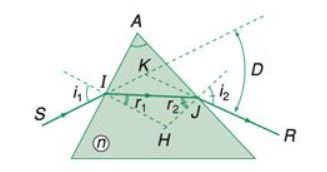
\includegraphics[scale=0.6]{../figs/VN11-2021-PH-TP037-01.JPG}
		\end{center}
	
	$$\sin i_1 = n \sin r; \sin i_2 = n \sin r_2.$$
	
	$$r_1 + r_2 = A.$$ 
	
	$$D = i_1 + i_2 -A.$$
	
	Góc lệch cực tiểu:

	$$ \sin \dfrac{D_\text m  + A}{2} = n \sin \dfrac{A}{2}.$$
	
	Vậy A, B, C đều đúng.
		
	}




	
	
	\item \mkstar{2} 
	
	\cauhoi{
	
	Một lăng kính đặt trong không khí, có góc chiết quang $A = 30^\circ$ nhận một tia sáng tới vuông góc với mặt bên AB và tia ló sát mặt bên AC của lăng kính. Chiết suất $n$ của lăng kính là
	
	\begin{mcq}(4)
		\item $\text{1,2}$.
		\item $\text{1,3}$.
		\item $\text{1,5}$.
		\item $\text{2,0}$.
	\end{mcq}
	}
	
	\loigiai{
		
	\textbf{Đáp án: D.}
	
	Tia tới vuông góc với mặt bên AB và tia ló sát mặt bên AC.
	
	$$ i_1 = 0^\circ; i_2 =90^\circ.$$
	
	Áp dụng công thức lăng kính
	
	$$\sin i_1  = n \sin r_1 \Rightarrow r_1 = 0^\circ.$$
	
	$$\Rightarrow r_2 = A - r_1 = 30^\circ.$$
	
	Lại có:
	
	$$\sin i_2 = n \sin r_2 \Rightarrow n = 2.$$
	}
	\item \mkstar{2} 
	
	\cauhoi{
		
		Tiết diện thẳng của đoạn lăng kính là tam giác đều. Một tia sáng đơn sắc chiếu tới mặt bên lăng kính và cho tia ló đi ra từ một mặt bên khác. Nếu góc tới và góc ló là $45^\circ$ thì góc lệch là
		\begin{mcq}(4)
			\item $10^\circ$.
			\item $20^\circ$.
			\item $30^\circ$.
			\item $40^\circ$
		\end{mcq}
	}
	
	\loigiai{
		
		\textbf{Đáp án: C.}
		
		
		Ta thấy $ i_1 = i_2 =45^\circ \Rightarrow $ tia sáng có góc lệch cực tiểu.
		
		Góc lệch cực tiểu giữa tia tới và tia ló
		
		$$D_\text{m} = 2i_\text{m} - A = 30^\circ.$$
		
	}

\end{enumerate}
\section{Thấu kính mỏng}
\begin{enumerate}[label=\bfseries Câu \arabic*:]
	
	\item \mkstar{2} 
	
	\cauhoi{
		
		Vật sáng nhỏ AB đặt vụông góc trục chính của một thấu kính và cách thấu kính 
		15 cm cho ảnh ảo lớn hơn vật hai lần. Tiêu cự của thấu kính là
		\begin{mcq}(4)
			\item 18 cm.
			\item 24 cm.
			\item 36 cm.
			\item 30 cm.
		\end{mcq}
	}
	
	\loigiai{
		
		\textbf{Đáp án: D.}
		
		Đối với thấu kính hội tụ vật thật đặt trong khoảng từ tiêu điểm đến thấu kính sẽ cho ảnh ảo lớn hơn vật.
		
		Do đó, thấu kính phải là thấu kính hội tụ.
		
		Tiêu cự của thấu kính 
		
		$$ k = - \dfrac{d'}{d} = - \dfrac{f}{d-f} \Rightarrow f = \SI{30}{cm}.$$
		
	
	}
	
	\item \mkstar{2}
	
	\cauhoi{
		Một thấu kính hội tụ có tiêu cự 30 cm. Vật sáng AB đặt vuông góc với trục chính của thấu kính. Ảnh của vật tạo hởi thấu kính ngược chiều với vật và cao gấp ba lần vật. Vật AB cách thấu kính 
		\begin{mcq}(4)
			\item 15 cm.
			\item 20 cm.
			\item 30 cm.
			\item 40 cm.
		\end{mcq}
	}
	\loigiai{
		
	\textbf{Đáp án: D.}
	
	Khoảng cách từ AB đến thấu kính
	
	$$ k = -\dfrac{d'}{d} = - \dfrac{f}{d - f} \Rightarrow d = \SI{40}{cm}.$$
	}

		\item \mkstar{3} 
	
	\cauhoi{
		
		Vật AB cao 2 cm đặt vuông góc với trục chính của thấu kính hội tụ cho ảnh A'B' cao 4cm. Tiêu cự thấu kính là $f=20\ \text{cm}$. Xác định vị trí của vật và ảnh.
		\begin{mcq}(2)
			\item $d=15\ \text{cm}, \ d'=-\text{30}\ \text{cm}$.
			\item $d=10\ \text{cm}, \ d'=-\text{20}\ \text{cm}$.
			\item $d=5\ \text{cm}, \ d'=-\text{10}\ \text{cm}$.
			\item $d=20\ \text{cm}, \ d'=-\text{40}\ \text{cm}$.
		\end{mcq}
	}
	
	\loigiai{
		\textbf{Đáp án: B.}
		
		Ta có:
		
		$$ k = - \dfrac{d'}{d} = 2 \Rightarrow d' + 2d = 0.\ (1)$$
		
		Lại có
		
		$$ f = \dfrac{dd'}{d + d'}.\ (2)$$
		
		Thay (1) vào (2) suy ra
		
		$$2d^2 -20d =0 \Rightarrow d =\SI{10}{cm}.$$
		
		Suy ra: $d' = -\SI{20}{cm}.$
		
		
		
		
	}
		\item \mkstar{3} 
	
	\cauhoi{
		
		Đặt một thấu kính cách một trang sách 20 cm, nhìn qua thấu kính thấy ảnh của dòng chữ cùng chiều với dòng chữ nhưng cao bằng một nửa dòng chữ thật. Tìm tiêu cự của thấu kính, suy ra thấu kính loại gì?
		
		\begin{mcq}(2)
			\item $f=-20\ \text{cm}$, thấu kính phân kỳ.
			\item $f=-10\ \text{cm}$, thấu kính phân kỳ.
			\item $f=20\ \text{cm}$, thấu kính hội tụ.
			\item $f=10\ \text{cm}$, thấu kính hội tụ.
		\end{mcq}
	}
	
	\loigiai{
		\textbf{Đáp án: A.}
		
		Nhìn qua thấu kính thấy ảnh của dòng chữ cùng chiều với dòng chữ nhưng cao bằng một nửa dòng chữ thật 
		
		$$k =\dfrac{1}{2} = - \dfrac{d'}{d} \Rightarrow d' = -\SI{10}{cm}.$$
		
		Ta có:
		
		$$\dfrac{1}{f} = \dfrac{1}{d} + \dfrac{1}{d'} \Rightarrow f = -\SI{20}{cm} < 0.$$
		
		Thấu kính là thấu kính phân kì.
	}
		\item \mkstar{3}
	
	\cauhoi{
		
		Một thấu kính hội tụ có tiêu cự 30 cm. Vật sáng AB đặt vuông góc với trục chính của thấu kính. Anh của vật tạo bởi thấu kính cùng chiều với vật và cao gấp hai lần vật. Vật AB cách thấu kính 
		\begin{mcq}(4)
			\item $10\ \text{cm}$.
			\item $45\ \text{cm}$.
			\item $15\ \text{cm}$.
			\item $90\ \text{cm}$.
		\end{mcq}
	}
	
	\loigiai{
		\textbf{Đáp án: C.}
		
		Vật đặt cách thấu kính
		
		$$ k = -\dfrac{f}{d-f} = 2\Rightarrow d = \SI{15}{cm}.$$ 
		
		(ảnh cùng chiều, trái bản chất với vật nên $k >0$).
	}
		\item \mkstar{3} 
	
	\cauhoi{
		
		Một thấu kính phân kì có độ tụ $-5\ \text{dp}$. Nếu vật sáng AB đặt vuông góc vói trục chính và cách thấu kính 30 cm thỉ ảnh cách vật một khoảng là $L$ với số phóng đại ảnh là $k$. Chọn phương án đúng.
		\begin{mcq}(4)
			\item $L = 20\ \text{cm}.$
			\item $k=-\text{0,4}.$
			\item $L = 40\ \text{cm}.$
			\item $k=\text{0,4}.$
		\end{mcq}
		
	}
	
	\loigiai{
		\textbf{Đáp án: D.}
		
		Ta có:
		
		$$ f = \dfrac{1}{D} = -\SI{0,2}{m}.$$
		
		Lại có:
		
		$$ d' = \dfrac{df}{d - f} = -12.$$
		
		Suy ra
		
		$$ L  =|d + d'| = \SI{18}{cm}.$$
		
		$$ k - \dfrac{d'}{d} = \SI{0,4}{}.$$
		
	}
		\item \mkstar{3}
	
	\cauhoi{
		Đặt vật sáng nhỏ AB vuông góc trục chính cua thấu kính có tiêu cự 16 cm, cho ảnh cao bằng nửa vật. Khoảng cách giữa vật và ảnh là
		\begin{mcq}(4)
			\item $72\ \text{cm}.$
			\item $80\ \text{cm}.$
			\item $30\ \text{cm}.$
			\item $90\ \text{cm}.$
		\end{mcq}
	}
	
	\loigiai{
		\textbf{Đáp án: A.}
		

		
		$$ k = - \dfrac{d'}{d} = -\dfrac{1}{2} \Rightarrow d' = \dfrac{1}{2} d.$$
		
		Lại có:
		
		$$\dfrac{1}{f} = \dfrac{1}{d} + \dfrac{1}{d'}.$$
		
		Suy ra $d =\SI{48}{cm}; d' = \SI{24}{cm}.$
		
		Vậy $L = |d + d'| = \SI{72}{cm}.$
		
	}
		\item \mkstar{3} 
	
	\cauhoi{
		
	Vật AB là đoạn thẳng sáng nhỏ đặt vuông góc với trục chính của một thấu kính cho ảnh ảo cao bằng 5 lần vật và cách vật 60 cm. Đầu A của vật nằm tại trục chính của thấu kính. Tiêu cực của thấu kính gần giá trị nào nhất sau đây?
	\begin{mcq} (4)
		\item $32\ \text{cm}.$
		\item $80\ \text{cm}.$
		\item $17\ \text{cm}.$
		\item $21\ \text{cm}.$
	\end{mcq}
	}
	
	\loigiai{
		\textbf{Đáp án: C.}
		
		Thấu kính phân kỳ, vật thật luôn cho ảnh ảo nhỏ hơn vật. Vậy thấu kính là thấu kính hội tụ và $k = + 5$.
		
		Ta có:
		
		$$ k = -\dfrac{d'}{d} = 5 \Rightarrow -d' =5d.$$
		
		Và $L = -(d+d') = \SI{60}{cm}.$
		
		Lại có:
		
		$$\dfrac{1}{f} = \dfrac{1}{d} + \dfrac{1}{d'} \Rightarrow f = \SI{18,75}{cm}.$$
	}
		\item \mkstar{3} 
	
	\cauhoi{
	Vật AB là đoạn thẳng sáng nhỏ vuông góc với trục chính của một thấu kính phân kì cho ảnh cao bằng $\text{0,5}$ lần vật và cách vật 60 cm. Đầu A của vật nằm tại trục chính của thấu kính. Tiêu cự của thấu kính gần giá trị nào nhất sau đây?
	\begin{mcq}(4)
		\item $-72\ \text{cm}.$
		\item $-80\ \text{cm}.$
		\item $-130\ \text{cm}.$ 
		\item $-90\ \text{cm}.$
	\end{mcq}
	}
	
	\loigiai{
		\textbf{Đáp án: C.}
		
		Thấu kính phân kì, vật thật luôn cho ảnh ảo cùng chiều và nhỏ hơn vật ($k = + \text{0,5}$).
		
		$$d = f - \dfrac{f}{k}; d '  = f - fk.$$
		
		Mà $k = \text{0,5}.$
		
		Suy ra $d = -f; d = \text{0,5}f.$
		
		Và $ L = d+ d'$
		
		Vậy $ f =-\SI{120}{cm}.$
	}
		\item \mkstar{3} 
	
	\cauhoi{
		
		 Một thấu kính hội tụ có tiêu cự $f = 20\ \text{cm}$. Vật sáng AB được đặt trước thấu kính và có ảnh A'B'. Cho biết khoảng cách vật và ảnh là 125 cm. Khoảng cách từ vật đến thấu kính là
		\begin{mcq}(2)
			\item 25 cm hoặc 100 cm.
			\item 20 cm hoặc 105 cm.
			\item 40 cm hoặc 85 cm hoặc 100 cm
			\item 25 cm hoặc 100 cm hoặc $\text{17,5}$ cm.
		\end{mcq}
	}
	
	\loigiai{
		\textbf{Đáp án: D.}
		
		Ta có: $$L =|d+d'|  \Rightarrow L = \left|d+ \dfrac{df}{d-f}\right|.$$
		
		+ Nếu $d + d' = \SI{125}{cm}$ thì $d^2 - 125d + 125f = 0.$
		
		$$\Rightarrow d =\SI{25}{cm}; d = \SI{100}{cm}.$$
		
		+ Nếu $d + d' = -\SI{125}{cm}$ thì $d^2 + 125d - 125f = 0.$
		
		$$\Rightarrow d =\SI{17,5}{cm}; d = \SI{-142,5}{cm}.$$
		
		
		
	}
		\item \mkstar{3}
	
	\cauhoi{
		Một vật sáng 4 mm đặt thẳng góc với trục chính của một thấu kính hội tụ (có tiêu cự 40 cm), cho ảnh cách vật 36 cm. Xác định tính chất, độ lớn của ảnh và vị trí của vật.
		\begin{mcq}
			\item Ảnh thật, cao 10 mm, cách thấu kính 24 cm.
			\item Ảnh ảo, cao 10 mm, vật cách thấu kính 24 cm.	
			\item Ảnh thật, cao 5 mm, vật cách thấu kính 12 cm.
			\item Ảnh ảo, cao 5 mm, vật cách thấu kính 12 cm.
		\end{mcq}
	}
	
	\loigiai{
		\textbf{Đáp án: B.}
		
	Ta có: $f = \SI{40}{cm}; L =\SI{36}{cm}.$
	
	Ta thấy $ L < f \Rightarrow $ ảnh ảo.
	
	$$\Rightarrow d + d' = - L = -\SI{36}{cm}\ (1).$$
	
	Lại có:
	
	$$\dfrac{1}{f} = \dfrac{1}{d} + \dfrac{1}{d'}.$$
	
	Từ (1) và (2) suy ra:
	
	$$ d = \SI{24}{cm}; d' = -\SI{60}{cm}.$$
	
	Độ phóng đại ảnh vật:
	
	$$ k = - \dfrac{d'}{d} = \text{2,5}.$$
	
	+ Vật thật cách thấu kính 24 cm.
	
	+ Ảnh ảo lớn hơn vật (gấp 2,5 lần vật), cách thấu kính 60 cm.
	}
		\item \mkstar{3} 
	
	\cauhoi{
		
		Một thấu kính hội tụ tiêu cự $f$. Đặt thấu kính này giữa vật AB và màn (song song với vật) sao cho ảnh cảu AB hiện rõ nét trên màn và gấp hai lần vật. Để ảnh rõ nét của vật trên màn gấp ba lần vật, phải tăng khoảng cách vật và màn thêm 10 cm.  Tiêu cự của thấu kính bằng
		\begin{mcq}(4)
			\item $12\ \text{cm}.$
			\item $20\ \text{cm}.$
			\item $17\ \text{cm}.$
			\item $15\ \text{cm}.$
		\end{mcq}
	}
	
	\loigiai{
		\textbf{Đáp án: A.}
		
		Ta có:
		
		$$ d = f - \dfrac{f}{k} ; d' = f- fk.$$
		
		Suy ra:
		
		$$ L =d + d' = 2f - \dfrac{f}{k}.$$
		
		Mà $k_1 =-2; k_2 = -3; L_2 - L_1 = \SI{10}{cm}.$
		
		$$\Rightarrow \dfrac{f}{3} + 3f - \dfrac{f}{2}-2f = 10 \Rightarrow f = \SI{12}{cm}.$$
		
	}
		\item \mkstar{3}
	
	\cauhoi{
		
		Vật sáng nhỏ AB đặt vuông góc trục chính của thấu kính. Khi vật cách thấu kính 30 cm thì cho ảnh thật $\text{A}_1\text{B}_1$. Đưa vật đến vị trí khác thì cho ảnh ảo $\text{A}_2\text{B}_2$ cách thấu kính 20 cm. Nếu hai ảnh $\text{A}_1\text{B}_1$ và $\text{A}_2\text{B}_2$ có cùng độ lớn thì tiêu cự của thấu kính bằng 
		\begin{mcq}(4)
			\item $18\ \text{cm}.$
			\item $15\ \text{cm}.$
			\item $20\ \text{cm}.$
			\item $30\ \text{cm}.$
		\end{mcq}
	}
	
	\loigiai{
		\textbf{Đáp án: C.}
		
		Vì đối với thấu kính phân kì vật thật luôn cho ảnh ảo do đó thấu kính chỉ có thể là thấu kính hội tụ.
		
		$$ k = -\dfrac{f}{d-f} = \dfrac{d'}{d-f'}.$$
		
		Mà $k_1 = -k_2.$
		
		$$\Rightarrow \dfrac{-f}{30-f} = \dfrac{-20 -f}{-f}.$$
		
		$$\Rightarrow f = -\SI{15}{cm}; f =\SI{20}{cm}.$$
	}
		\item \mkstar{3} 
	
	\cauhoi{
		Một vật sáng phẳng đặt trước một thấu kính, vuông góc với trục chính. Ảnh của vật tạo bởi thấu kính bằng ba lần vật. Dời vật lại gần thấu kính một đoạn 12 cm. Ảnh của vật ở vị trí mới vẫn bằng ba lần vật. Tiêu cự của thấu kính gần giá trị nào nhất sau đây? 
		\begin{mcq} (4)
			\item $10\ \text{cm}.$
			\item $20\ \text{cm}.$
			\item $30\ \text{cm}.$
			\item $40\ \text{cm}.$
		\end{mcq}
	}
	
	\loigiai{
		\textbf{Đáp án: B.}
		
		+ Thấu kính phân kì vật thật luôn cho ảnh ảo nhỏ hơn vật. Thấu kính hội tụ vật thật đặt trong tiêu cự cho ảnh ảo lớn hơn vật, vật thật đặt đặt cách thấu kính từ $f$ đến $2f$ cho ảnh thật lớn hơn vật, và vật thật đặt cách thấu kính lớn hơn $2f$ cho ảnh thật nhỏ hơn vật.
		
		+ Hai ảnh có cùng độ lớn thì một ảnh là ảnh thật (ảnh đầu) và một ảnh là ảnh ảo (ảnh sau).
		
		$$\dfrac{1}{f} = \dfrac{1}{d} + \dfrac{1}{d'}.$$
		
		$$ k = -\dfrac{d'}{d}.$$
		
	
		
		$$\Rightarrow d = f - \dfrac{d}{k}; d' = f - fk.$$
		
		$$\Rightarrow d_1 = f - \dfrac{f}{-3}; d_2 = f - \dfrac{f}{+3}.$$
		
		Mà $d_1 - d_2 =12.$ nên
		
		$$\Rightarrow f = \SI{18}{cm}.$$
		
		
		
		
	}
		\item \mkstar{3} 
	
	\cauhoi{
		
		Một vật thật AB đặt vuông góc với trục chính của một thấu kính. Ban đầu ảnh của vật qua thấu kính là ảnh ảo và bằng nửa vật. Giữ thấu kính cố định di chuyển vật dọc trục chính 100 cm. Ảnh của vật vẫn là ảnh ảo và cao bằng $\dfrac{1}{3}$ vật. Xác định chiều dời của vật, vị trí ban đầu của vật và tiêu cự của thấu kính?
		\begin{mcq} 
			\item Vật ra xa thấu kính, vị trí ban đầu cách thấu kính 100 cm, tiêu cự $f=-100\ \text{cm}.$ 
			\item Vật lại gần thấu kính, vị trí ban đầu cách thấu kính 100 cm, tiêu cự $f=-100\ \text{cm}.$ 
			\item Vật ra xa thấu kính, vị trí ban đầu cách thấu kính 50 cm, tiêu cự $f=-50\ \text{cm}.$ 
			\item Vật lại gần thấu kính, vị trí ban đầu cách thấu kính 50 cm, tiêu cự $f=-50\ \text{cm}.$ 
		\end{mcq}
	}
	
	\loigiai{
		\textbf{Đáp án: A.}
		
		Vật qua thấu kính cho ảnh ảo nhỏ hơn vật nên thấu kính là thấu kính phân kì
		
		$$ - \dfrac{d'_1}{d_1} = \dfrac{1}{2} \Rightarrow d_1 = - 2d'_1 = 2 \dfrac{d_1f}{f - d_1} \Rightarrow d_1 =-f.$$
		
		$$ - \dfrac{d'_2}{d_2} = \dfrac{1}{3} \Rightarrow d_2 = - 3d'_2 = 3\dfrac{d_2f}{f - d_2} \Rightarrow d_2 =-2f.$$
		
		Do $f < 0$ nên $d_2 >d_1$, ta có $d_2 = d_1 + 100.$
		
		Suy ra: $ -2f = -f +100 \Rightarrow f = -\SI{100}{cm}.$
	}
	
\end{enumerate}
\section{Mắt}
\begin{enumerate}[label=\bfseries Câu \arabic*:]
	
	\item \mkstar{1} 
	
	\cauhoi{
		
		Điểm cực viễn ($C_V$) của mắt là
		\begin{mcq}
			\item Khi mắt không điều tiết, điểm gần nhất trên trục của mắt cho ảnh trên võng mạc.
			\item Khi mắt điều tiết tối đa, điểm xa nhất trên trục của mắt cho ảnh trên võng mạc.
			\item Khi mắt điều tiết tối đa, điểm gần nhất trên trục của mắt cho ảnh trên võng mạc.
			\item Khi mắt không điều tiết, điểm xa nhất trên trục của mắt cho ảnh trên võng mạc.
		\end{mcq}
	}
	
	\loigiai{
		\textbf{Đáp án: D.}
		
		Điểm cực viễn: Điểm xa nhất trên trục chính của mắt mà đặt vật tại đó mắt có thể thấy rõ được mà không cần điều tiết, ($f = f_\text{max}$).
		
		Khi quan sát vật ở $C_V$ mắt không phải điều tiết nên mắt không mỏi.
		
	
	}
		\item \mkstar{1} 
	
	\cauhoi{
		
		Điểm cực cận ($C_C$) của mắt là
		\begin{mcq}
			\item Khi mắt không điều tiết, điểm gần nhất trên trục của mắt cho ảnh trên võng mạc.
			\item Khi mắt điều tiết tối đa, điểm gần nhất trên trục của mắt cho ảnh trên võng mạc.
			\item Khi mắt điều tiết tối đa, điểm xa nhất trên trục của mắt cho ảnh trên võng mạc.
			\item Khi mắt không điều tiết, điểm xa nhất trên trục của mắt cho ảnh trên võng mạc.
		\end{mcq}
	}
	
	\loigiai{
		\textbf{Đáp án: B.}
		
		Điểm cực cận: Điểm gần nhất trên trục chính của măt mà đặt vật tại đó mắt có thể thấy rõ được khi đã điều tiết tối đa ($f = f_\text{min}$).
		
		
	}
	
	\item \mkstar{3} 
	
	\cauhoi{
		Một người có thể nhìn rõ các vật cách mắt từ $\SI{10}{\centi\meter}$ đến $\SI{100}{\centi\meter}$. Độ biến thiên độ tụ của mắt người đó từ trạng thái không điều tiết đến trạng thái điều tiết tối đa là
		\begin{mcq}(4)
			\item $\SI{12}{dp}$.
			\item $\SI{5}{dp}$.
			\item $\SI{6}{dp}$.
			\item $\SI{9}{dp}$.
		\end{mcq}
	}
	
	\loigiai{
		\textbf{Đáp án: D.}
		
		+ Khi quan sát trong trạng thái không điều tiết:
		
		$$D_\text{min} = \dfrac{1}{f_\text{max}} = \dfrac{1}{OC_V} + \dfrac{1}{OV}.$$
		
		+ Khi quan sát trong trạng thái điều tiết tối đa: 
		
		$$D_\text{max} = \dfrac{1}{f_\text{max}} = \dfrac{1}{OC_C} + \dfrac{1}{OV}.$$
		
		
		+ Độ biến thiên độ tụ:
		
		$$\Delta D  = D_\text{max} -  D_\text{min} = \SI{9}{dp}.$$
	}
	
	\item \mkstar{3} 
	
	\cauhoi{
		
		Một người có thể nhìn rõ các vật cách mắt $\SI{12}{\centi\meter}$ thì mắt không phải điều tiết. Lúc đó, độ tụ của thuỷ tinh thể là $\SI{62,5}{dp}$. Khoảng cách từ quang tâm thuỷ tinh thể đến võng mạc \textbf{gần giá trị nào nhất} sau đây?
		\begin{mcq}(4)
			\item $\SI{1,8}{\centi\meter}$.
			\item $\SI{1,5}{\centi\meter}$.
			\item $\SI{1,6}{\centi\meter}$.
			\item $\SI{1,9}{\centi\meter}$.
		\end{mcq}
		
	}
	\loigiai{
		
		\textbf{Đáp án: A.}
		
		+ Khi quan sát trong trạng thái không điều tiết:
		
		$$D_\text{min} = \dfrac{1}{f_\text{max}} = \dfrac{1}{OC_V} + \dfrac{1}{OV} \Rightarrow OV  = \SI{0,018}{m}.$$
		}
	
	\item \mkstar{3}
	
	\cauhoi{
		
		Một người mắt không có tật, quang tâm nằm cách võng mạc một khoảng $\SI{2,2}{\centi\meter}$. Độ tụ của mắt khi quan sát không điều tiết \textbf{gần giá trị nào nhất} sau đây?
	\begin{mcq}(4)
		\item $\SI{42}{dp}$.
		\item $\SI{45}{dp}$.
		\item $\SI{46}{dp}$.
		\item $\SI{49}{dp}$.
	\end{mcq}
		
	}
	\loigiai{
		
	\textbf{Đáp án: B.}
	
+ Khi quan sát trong trạng thái không điều tiết:

$$D_\text{min} = \dfrac{1}{f_\text{max}} = \dfrac{1}{OC_V} + \dfrac{1}{OV}  = \SI{45,45}{dp}.$$
	
	}

		\item \mkstar{3} 
	
	\cauhoi{
		
		Một người mắt không có tật, quang tâm nằm cách võng mạc một khoảng $\SI{2,2}{\centi\meter}$. Độ tụ của mắt đó khi quan sát một vật cách mắt $\SI{20}{\centi\meter}$ \textbf{gần giá trị nào nhất} sau đây?
	\begin{mcq}(4)
		\item $\SI{42}{dp}$.
		\item $\SI{45}{dp}$.
		\item $\SI{46}{dp}$.
		\item $\SI{49}{dp}$.
	\end{mcq}
	}
	
	\loigiai{
		\textbf{Đáp án: D.}
		
		Khi quan sát một vật cách mắt:
		
		$$D = \dfrac{1}{d} + \dfrac{1}{OV} = \SI{50,45}{dp}.$$
	}
		\item \mkstar{3} 
	
	\cauhoi{
		Mắt của một người có quang tâm cách võng mạc khoảng $\SI{1,52}{\centi\meter}$. Tiêu cự thể thủy tinh thay đổi giữa hai giá trị $f_1=\SI{1,500}{\centi\meter}$ và $f_2=\SI{1,415}{\centi\meter}$. Khoảng nhìn rõ của mắt \textbf{gần giá trị nào nhất} sau đây?
		\begin{mcq}(4)
			\item $\SI{95,8}{\centi\meter}$.
			\item $\SI{93,5}{\centi\meter}$.
			\item $\SI{97,4}{\centi\meter}$.
			\item $\SI{97,8}{\centi\meter}$.
		\end{mcq}
	}
	
	\loigiai{
		\textbf{Đáp án: B.}
		
		$$\dfrac{1}{OC_V} = \dfrac{1}{f_\text{max}} - \dfrac{1}{OV} \Rightarrow OC_V = \SI{114}{cm}.$$
		
		$$\dfrac{1}{OC_C} = \dfrac{1}{f_\text{min}} - \dfrac{1}{OV} \Rightarrow OC_C = \SI{20,5}{cm}.$$
		
		Khoảng nhìn rõ: 
		
		$$C_VC_C = 114 - \text{20,5} = \SI{93,5}{cm}.$$
	}
		\item \mkstar{3} 
	
	\cauhoi{
	
		Mắt của một người có điểm cực viễn cách mắt $\SI{80}{\centi\meter}$. Muốn nhìn thấy vật ở vô cực không điều tiết, người đó phải đeo kính sát mắt có độ tụ
		\begin{mcq}(4)
			\item $\SI{-4}{dp}$.
			\item $\SI{-1,25}{dp}$.
			\item $\SI{-2}{dp}$.
			\item $\SI{-2,5}{dp}$.
		\end{mcq}
	}
	
	\loigiai{
		\textbf{Đáp án: B.}
		
		Người đó đeo kính phân kì để nhìn rõ các vật ở vô cực mà mắt không phải điều tiết (vật ở vô cùng qua Ok cho ảnh ảo nằm tại điểm cực viễn $C_V$)
		
		$$f_k = -\SI{0,8}{m}.$$
		
		Độ tụ của kính
		
		$$D_k = \dfrac{1}{f_k} = - \SI{1,25}{dp}.$$
		
	}
		\item \mkstar{3}
	
	\cauhoi{
		Một người khi không đeo kính có thể nhìn rõ các vật gần nhất cách mắt $\SI{50}{\centi\meter}$. Xác định độ tụ của kính mà người đó cần đeo sát mắt để có thể nhìn rõ các vật gần nhất cách mắt $\SI{25}{\centi\meter}$.
		\begin{mcq}(4)
			\item $\SI{4,2}{dp}$.
			\item $\SI{2}{dp}$.
			\item $\SI{3}{dp}$.
			\item $\SI{1,9}{dp}$.
		\end{mcq}
	}
	
	\loigiai{
		\textbf{Đáp án: B.}
		
		+ Để khi đeo kính nhìn được vật gần nhất cách mắt 25 cm thì qua kính cho một ảnh ảo tại điểm cực cận của mắt.
		
		$$ d = \SI{25}{cm}; d' = -OC_C.$$
		
		$$f = \dfrac{dd'}{d+d'} = \SI{50}{cm}.$$
		
		Độ tụ của kính
		
		$$D = \dfrac{1}{f} = \SI{2}{dp}.$$
	}
		
		\item \mkstar{3} 
	
	\cauhoi{
		
		Một người cận thị phải kính sát mắt có độ tụ $\SI{-2,5}{dp}$. Khi đeo kính đó, người ấy có thể nhìn rõ các vật gần nhất cách kính $\SI{24}{\centi\meter}$. Khoảng nhìn rõ của mắt khi không đeo kính \textbf{gần giá trị nào nhất} sau đây?
		\begin{mcq}(4)
			\item $\SI{26}{\centi\meter}$.
			\item $\SI{15}{\centi\meter}$.
			\item $\SI{50}{\centi\meter}$.
			\item $\SI{40}{\centi\meter}$.
		\end{mcq}
	}
	
	\loigiai{
		\textbf{Đáp án: A.}
		
		Ta có:
		
		$$ \dfrac{1}{d_C} + \dfrac{1}{- OC_C} = D_k.$$
		
		$$ \dfrac{1}{d_V} + \dfrac{1}{- OC_V} = D_k.$$
		
		Suy ra: $OC_C =\SI{0,15}{m}, OC_V = \SI{0,4}{m}.$
		
		Khoảng nhìn rõ của mắt khi không đeo kính 
		
		$$C_CC_V = OC_V - OC_C =\SI{0,25}{m}.$$
	}
\end{enumerate}	
\section{Kính lúp}
\begin{enumerate}[label=\bfseries Câu \arabic*:]
	
		\item \mkstar{1} 
	
	\cauhoi{
		
		Kính lúp là dụng cụ quang dùng để
		\begin{mcq}
			\item bổ trợ cho mắt làm tăng góc trông của các vật nhỏ.
			\item tạo ra một ảnh thật, lớn hơn vật và thu trên màn để quan sát vật rõ hơn.
			\item bổ trợ cho mắt cận thị quan sát được những vật ở rất xa.
			\item tạo ra một ảnh thật, lớn hơn vật và trong giới hạn nhìn rõ của mắt.
		\end{mcq}
	}
	
	\loigiai{
		\textbf{Đáp án: A.}
		
		Kính lúp là một công cụ quang phổ học bổ trợ cho mắt việc quan sát các vật nhỏ. Nó có tác dụng làm tăng góc trông ảnh bằng cách tạo ra một ảnh ảo, lớn hơn vật và nằm trong giới hạn thấy rõ của mắt.
	}
	\item \mkstar{1} 
	
	\cauhoi{
		
		Khi nói về kính lúp, phát biểu nào sau đây là sai?
		\begin{mcq}
			\item kính lúp là dụng cụ quang bổ trợ cho mắt làm tăng góc trông quan sát các vật nhỏ.
			\item Vật cần quan sát đặt trước kính lớp cho ảnh ảo có số phóng đại lớn.
			\item Kính lúp đơn giản là một thấu kính hội tụ có tiêu cự ngắn.
			\item Vật cần quan sát đặt trước kính lúp cho ảnh thật có số phóng đại lớn.
		\end{mcq}
	}
	
	\loigiai{
		\textbf{Đáp án: D.}
		
		Vật cần quan sát đặt trước kính lúp cho ảnh ảo có số phóng đại lớn.
		
		
	}
	\item \mkstar{2} 
	
	\cauhoi{
		
		Một mắt không có tật có điểm cực cận cách mắt $\SI{20}{\centi\meter}$, quan sát vật AB qua một kính lúp có tiêu cực $\SI{2}{\centi\meter}$. Xác định số bội giác của kính lúp khi ngắm chừng ở vô cực
	\begin{mcq}(4)
		\item 6.
		\item 10.
		\item 15.
		\item 2,5.
	\end{mcq}
	}
	
	\loigiai{
		\textbf{Đáp án: B.}
		
		Số bội giác của kính lúp ngắm chừng ở vô cực
		
		$$\text G = \dfrac{\text{OC}_\text C}{f}= 10.$$
	}
	
	\item \mkstar{2} 
	
	\cauhoi{
		Một kính lúp là một thấu kính hội tụ có độ tụ $\SI{10}{dp}$. Mắt người quan sát có khoảng nhìn rõ ngắn nhất là $\SI{20}{\centi\meter}$. Độ bội giác của kính lúp khi ngắm chừng ở vô cực là 
	\begin{mcq}(4)
		\item 2,5.
		\item 4.
		\item 5.
		\item 2.
	\end{mcq}
	}
	\loigiai{
		\textbf{Đáp án: D.}
		
		Độ bội giác khi ngắm chừng ở vô cực 
		
		$$\text G = \dfrac{\text{OC}_\text C}{f}= D \cdot \text{OC}_\text C = 2.$$
	}
	
	\item \mkstar{2}
	
	\cauhoi{
		
		Một học sinh, có mắt không bị tật, có khoảng cực cận $\text{OC}_\text{C}=\SI{25}{\centi\meter}$, dùng kính lúp có độ tụ $+\SI{10}{dp}$ để quan sát một vật nhỏ. Biết ngắm chừng kính lúp ở vô cực. Tính số bội giác. 
		\begin{mcq}(4)
			\item 6.
			\item 4.
			\item 15.
			\item 2,5.
		\end{mcq}
		
	}
	\loigiai{
		
		\textbf{Đáp án: D.}
		
	$$\text G = \dfrac{\text{OC}_\text C}{f}= D \cdot \text{OC}_\text C = \text{2,5}.$$
	}


		\item \mkstar{2} 
	
	\cauhoi{
			Một mắt không tật có điểm cực cận cách mắt $\SI{20}{\centi\meter}$, quan sát vật AB qua một kính lúp có tiêu cự $\SI{2}{\centi\meter}$. Xác định số bội giác của kính khi ngắm chừng ở điểm cực cận, khi mắt đặt tại tiêu điểm ảnh của kính.
		\begin{mcq}(4)
			\item 6.
			\item 4.
			\item 10.
			\item 2,5.
		\end{mcq}
	}
	
	\loigiai{
		\textbf{Đáp án: B.}
		
			$$\text G = \dfrac{\text{OC}_\text C}{f} = 10.$$
	}
		
		\item \mkstar{2} 
	
	\cauhoi{
			Trong các kính lúp sau, kính lúp nào khi dùng để quan sát một vật sẽ cho ảnh lớn nhất?
		\begin{mcq}(2)
			\item Kính lúp có số bội giác $G = 5$.
			\item Kính lúp có số bội giác $G = 1,5$.
			\item Kính lúp có số bội giác $G = 6$.
			\item Kính lúp có số bội giác $G = 4$.
		\end{mcq}
	}
	
	\loigiai{
		\textbf{Đáp án: C.}
		
		Ta có: Kính lúp có độ bội giác càng lớn thì quan sát ảnh càng lớn.
		
		Phương án C có độ bội giác lớn nhất trong các phương án là G = 6 sẽ cho ảnh lớn nhất
	}
		\item \mkstar{2} 
	
	\cauhoi{
			Thấu kính hội tụ có tiêu cự nào sau đây không thể dùng làm kính lúp?
		\begin{mcq}(4)
			\item $\SI{25}{\centi\meter}$.
			\item $\SI{14}{\centi\meter}$.
			\item $\SI{3}{\centi\meter}$.
			\item $\SI{9}{\centi\meter}$. 
		\end{mcq}
	}
	
	\loigiai{
		\textbf{Đáp án: A.}
		
		Tiêu cự của kính lúp phải nhỏ hơn 25 cm. Nên thấu kính hội tụ có tiêu cự 25 cm không dùng để làm kính lúp được.
	}
		\item \mkstar{3} 
	
	\cauhoi{
	Dùng kính lúp có số bội giác $G=2,5x$ để quan sát một vật nhỏ cao $\SI{2}{\milli\meter}$. Muốn có ảnh ảo cao $\SI{8}{\milli\meter}$ thì phải đặt vật cách kính bao nhiêu? Lúc đó ảnh cách kính bao?
	\begin{mcq}(4)
		\item $\SI{30}{\centi\meter}$.
		\item $\SI{25}{\centi\meter}$.
		\item $\SI{20}{\centi\meter}$.
		\item $\SI{15}{\centi\meter}$. 
	\end{mcq}
	}
	
	\loigiai{
		\textbf{Đáp án: A.}
		
		Tiêu cực của kính lúp
		
		$$ \text G = \dfrac{25}{f} \Rightarrow f = \SI{10}{cm}.$$
		
		Để ảnh của vật 10 mm thì hệ số phóng đại của ảnh phải là $k$ = 4.
		
		$$ k = \dfrac{d'}{d} =4.$$
		
		Kính lúp là thấu kính hội tụ có tiêu cự 10 cm. Áp dụng công thức thấu kính cho trường hợp ảnh ảo ta có
		
		$$\dfrac{1}{d} = \dfrac{1}{f} - \dfrac{1}{d'} \Rightarrow d = \dfrac{3f}{4} \SI{7,5}{cm}.$$
		
		Khoảng cách từ ảnh đến kính lúp là: $\text{7,5}\cdot 4 = \SI{30}{cm}.$
		
		
		Vậy kính lúp đặt cách vật 7,5 cm, và cách ảnh 30 cm.
	}
		\item \mkstar{3} 
	
	\cauhoi{
		Trên vành của một chiếc kính lúp có ghi $G = 5x$. Vật nhỏ S có chiều cao là $\SI{0,4}{\centi\meter}$ được đặt trước kính lúp và cách kính lúp $\SI{3}{\centi\meter}$. Ảnh của S qua kính lúp cách S bao nhiêu?
		\begin{mcq}(4)
			\item $\SI{4,5}{\centi\meter}$.
			\item $\SI{2}{\centi\meter}$.
			\item $\SI{1,5}{\centi\meter}$.
			\item $\SI{1}{\centi\meter}$. 
		\end{mcq}	
	}
	
	\loigiai{
		\textbf{Đáp án: A.}
		
		Tiêu cự của kính lúp là:
		
		$$ \text G  = \dfrac{25}{f} \Rightarrow f = \SI{5}{cm}.$$
		
		Vì $d < f$ nên ảnh này là ảnh ảo, nằm cùng phía với vật so với kính lúp
		
		
		Áp dụng công thức thấu kính hội tụ với ảnh ảo
		
		$$\dfrac{1}{d'}= \dfrac{1}{f} - \dfrac{1}{d} \Rightarrow d' = \SI{7,5}{cm}.$$
		
		Khoảng cách từ ảnh đến vật là
		
		$$\text{7,5} - 3 = \text{4,5}\ \text{cm}.$$
	}
		
\end{enumerate}	
\whiteBGstarEnd